\documentclass[10pt]{article}
\usepackage[utf8]{inputenc}
\usepackage[activeacute,spanish]{babel}
\usepackage[left=1.5cm,top=1.5cm,right=1.5cm, bottom=1.5cm,letterpaper, includeheadfoot]{geometry}

\usepackage{amssymb, amsmath, amsthm}
\usepackage{graphicx}
\usepackage{hyperref}
\usepackage{lmodern,url}
\usepackage{paralist} %util para listas compactas
\usepackage{xcolor}
\usepackage{bbm}
\usepackage{mathrsfs}
\usepackage{bbm}

%========PAQUETES AGREGADOS===========
%Pseudocodigo
\usepackage{pseudocode}
\usepackage[portuguese, boxruled]{algorithm2e}
\usepackage{wrapfig}
\usepackage{multicol}
\usepackage{graphicx}
\usepackage{caption}
\usepackage{subcaption}
%\captionsetup[table]{labelformat=empty}
\captionsetup[subfigure]{labelformat=empty}
\usepackage{cancel}
\usepackage{tikz}
\def\checkmark{\tikz\fill[scale=0.4](0,.35) -- (.25,0) -- (1,.7) -- (.25,.15) -- cycle;} 
%====================================

\usepackage{fancyhdr}
\pagestyle{fancy}
\fancypagestyle{plain}{%
\fancyhf{}
\lhead{\footnotesize\itshape\bfseries\rightmark}
\rhead{\footnotesize\itshape\bfseries\leftmark}
}


% macros
\newcommand{\Q}{\mathbb Q}
\newcommand{\R}{\mathbb R}
\newcommand{\N}{\mathbb N}
\newcommand{\Z}{\mathbb Z}
\newcommand{\C}{\mathbb C}
\newcommand{\BigO}{\mathcal{O}}
%Teoremas, Lemas, etc.
\theoremstyle{plain}
\newtheorem{teo}{Teorema}
\newtheorem{lem}{Lema}
\newtheorem{prop}{Proposición}
\newtheorem{cor}{Corolario}
\newtheorem{obs}{Observación}
\newtheorem{ej}{Ejemplo}
\renewcommand{\qedsymbol}{\rule{0.7em}{0.7em}}
\renewenvironment{proof}{{\bfseries \noindent Demostración}}{ \qed \\}


\theoremstyle{definition}
\newtheorem{defi}{Definición}
% fin macros


\newcommand{\catnum}{23} %numero de catedra
\newcommand{\fecha}{1 de Diciembre 2016 }

%%%%%%%%%%%%%%%%%%

%Macros para este documento
\newcommand{\cin}{\operatorname{cint}}



\begin{document}
%Encabezado
\fancyhead[L]{Facultad de Ciencias Físicas y Matemáticas}
\fancyhead[R]{Universidad de Chile}
\vspace*{-1.2 cm}
\begin{minipage}{0.6\textwidth}
\begin{flushleft}
\hspace*{-0.5cm}\textbf{MA3402-1 Estadística. Primavera 2016}\\
\hspace*{-0.5cm}\textbf{Profesor:} Raul Gouet\\
\hspace*{-0.5cm}\textbf{Escriba:} Manuel Cáceres\\
\hspace*{-0.5cm}\textbf{Fecha:} \fecha
\end{flushleft}
\end{minipage}
\begin{minipage}{0.36\textwidth}
\begin{flushright}

\includegraphics[scale=0.3]{imagenes/fcfm_dcc}
\end{flushright}
\end{minipage}
\bigskip
%Fin encabezado

\begin{center}
\LARGE\textbf{Clase \catnum}
\end{center}
Tenemos la hipótesis de normalidad
\begin{align*}
\epsilon \sim NM(0,\sigma^2I)\\
Y = X\beta + \epsilon, rg(X) = k\ (completo)
\end{align*}
Gracias a esta hipótesis $\hat{\beta}$ resulta EIVUM y $\hat{\beta} \sim NM(\beta , \sigma^2(XX')^{-1})$. En particular, $\forall$ combinación lineal de los $\hat{\beta}$ es también normal, por ejemplo $\hat{\phi} = a'\hat{\beta}$ ( estimador insesgado de $\phi = a'\beta$) es normal $N(a'\beta , \sigma^2 a'(X'X)^{-1}a)$. Podemos hacer intervalos de confianza para $\phi$ siendo $\sigma$ conocido o no. Si $\sigma$ es conocido usamos el pivote:
\begin{align*}
\frac{\hat{\phi}-\phi}{\sigma\sqrt{a'(X'X)^{-1}a}} \sim N(0,1)
\end{align*}
En particular, si $a = e_{j} = \begin{bmatrix}
0_{1}\\ \ldots \\
1_{j} \\ \ldots \\ 0_{n}\end{bmatrix}$, obtenemos intervalos para cada $\beta_{j}$ en $\beta$.\\
Si $\sigma$ es desconocido entonces se aprovecha lo siguiente:
\begin{align*}
\frac{\hat{\sigma}^2}{\sigma^2} = \frac{||\hat{\epsilon}||^2}{\sigma^2} \sim \chi^2 (n-k)
\end{align*}
independiente de $\hat{\beta}-\beta$.\\

Entonces podemos cambiar en el pivote $\sigma^2$ por $\hat{\sigma}^2 = \frac{1}{n-k}||\hat{\epsilon}||^2$ y tenemos una $t(n-k)$.\\

Con la normalidad podemos resolver ciertos problemas de test de hipótesis. En particular, hipótesis lineales.\\

Por ejemplo $H_{0}\colon \beta = 0$ versus $H_{1}\colon \beta \not = 0$, $\beta = \begin{bmatrix}
\beta_{1}\\ \ldots \\ \beta_{2}
\end{bmatrix}$.\\

Notar que $\beta = 0 \Leftrightarrow$ no hay modelo lineal en esas variables $X$ ( puede existir con otros o ser no lineal). \\

Otro ejemplo es: Supongamos $X = [X_{1},X_{2}], X_{1}, X_{2}$ submatrices de $X$. Entonces podemos escribir
\begin{align*}
Y=X_{1}\beta_{1}+ X_{2}\beta_{2}+\epsilon
\end{align*}
con $\beta = \begin{bmatrix}
\beta_{1}\\ \beta_{2}
\end{bmatrix}$.\\

Planteamos $H_{0}\colon \beta_{1}=0$ versus $H_{1}\colon \beta_{1} \not = 0$.\\

Si aceptamos $H_{0}$, podemos descartar las variables en $X_{1}$.\\

Un último ejemplo $H_{0}\colon \beta_{1}=\beta_{2}$ versus $H_{1}\colon \beta_{1}\not = \beta_{2}$, $\beta = \begin{bmatrix}
\beta_{1}\\ \beta_{2} \\ \ldots \\ \beta_{k}
\end{bmatrix}$ o bien $H_{0} \colon a_{1}\beta_{1} + a_{2}\beta_{2} + a_{3}\beta_{3} = 0$ versus $H_{1}\colon no$.\\

La hipótesis lineal general tiene la forma siguiente: $H_{0}\colon H\beta = 0$, donde $H$ es una matriz (determinada, conocida) con $q$ filas y $k$ columnas, de rango completo $(q\le k)$, es decir $rg(H) = q$. Por cierto, $H_{1}\colon H\beta \not = 0$.\\

Una idea natural, es aplicar TRV. Definimos $\lambda$ como
\begin{align*}
\lambda = \frac{\sup_{\theta\in\Theta_{1}} f_{\theta}(y)}{\sup_{\theta\in\Theta_{0}}f_{\theta}(y)}
\end{align*}

Rechazamos $H_{0}$ si $\lambda(y) \ge k_{\alpha}$ ($k_{\alpha}$ se calcula con la ley bajo $H_{0}$, de forma que el nivel de significación sea $\alpha$).
\begin{align*}
\Theta = \{\theta = (\beta,\sigma)\colon \beta \in \mathbb{R}^k, \sigma > 0 \},\ \Theta_{0} = \{(\beta,\sigma)\in \Theta \colon H\beta = 0\}
\end{align*}
Recordemos que $Y \sim NM(X\beta, \sigma^2I)$, por lo tanto
\begin{align*}
f_{\theta} = \frac{1}{(2\pi)^{n/2}\sigma^n}e^{-1/2\sigma^2 (y- X\beta)'(y-X\beta)}
\end{align*}
\begin{align*}
\sup_{\theta\in \Theta} f_{\theta}(y) = f_{\hat{\theta}} &\quad \hat{\theta}\ EMV\ de\ \theta= (\hat{\beta},\hat{\sigma})\\
&\quad \hat{\beta} = (X'X)^{-1}X'Y\\
&\quad \hat{\sigma}^2 = \frac{1}{n}(Y-X\hat{\beta})'(Y-X\hat{\beta}) = \frac{||\hat{\epsilon}||^2}{n}\\
f_{\hat{\theta}}(y) = k \hat{\sigma}^{-n}\\
\sup_{\theta\in\Theta_{0}} = f_{\tilde{\theta}}(y) &\quad \tilde{\theta} = (\tilde{\beta},\tilde{\sigma})
\end{align*}
donde $\tilde{\beta}$ es solución de $\min_{\beta} (Y-X\beta)'(Y-X\beta)$ s.a. $H\beta= 0$.\\

$\tilde{\beta}$ existe porque, de hecho $X\hat{\beta}$ es la proyección ortogonal de $Y$ en cierto subespacio vectorial de $<X>$.\\

Definamos $<X>_{0} = \{X\beta \colon \beta \in \mathbb{R}^k, H\beta = 0\}$. Por cierto $<X>_{0}\subseteq <X>$ y además es subespacio vectorial.\\

Nuestro problema de minimización equivale a proyectar $Y$ en $<X>_{0}$ ortogonal y eso existe, claro.\\

Así $f_{\tilde{\theta}} (y) = k \tilde{\sigma}^{-n} \Rightarrow \lambda(y) = \left(\frac{\tilde{\sigma}^2}{\hat{\sigma}^2}\right)^{n/2}$. Rechazamos $H_{0}$ si $\frac{\tilde{\sigma}}{\hat{\sigma}}$ es muy grande.
\begin{center}
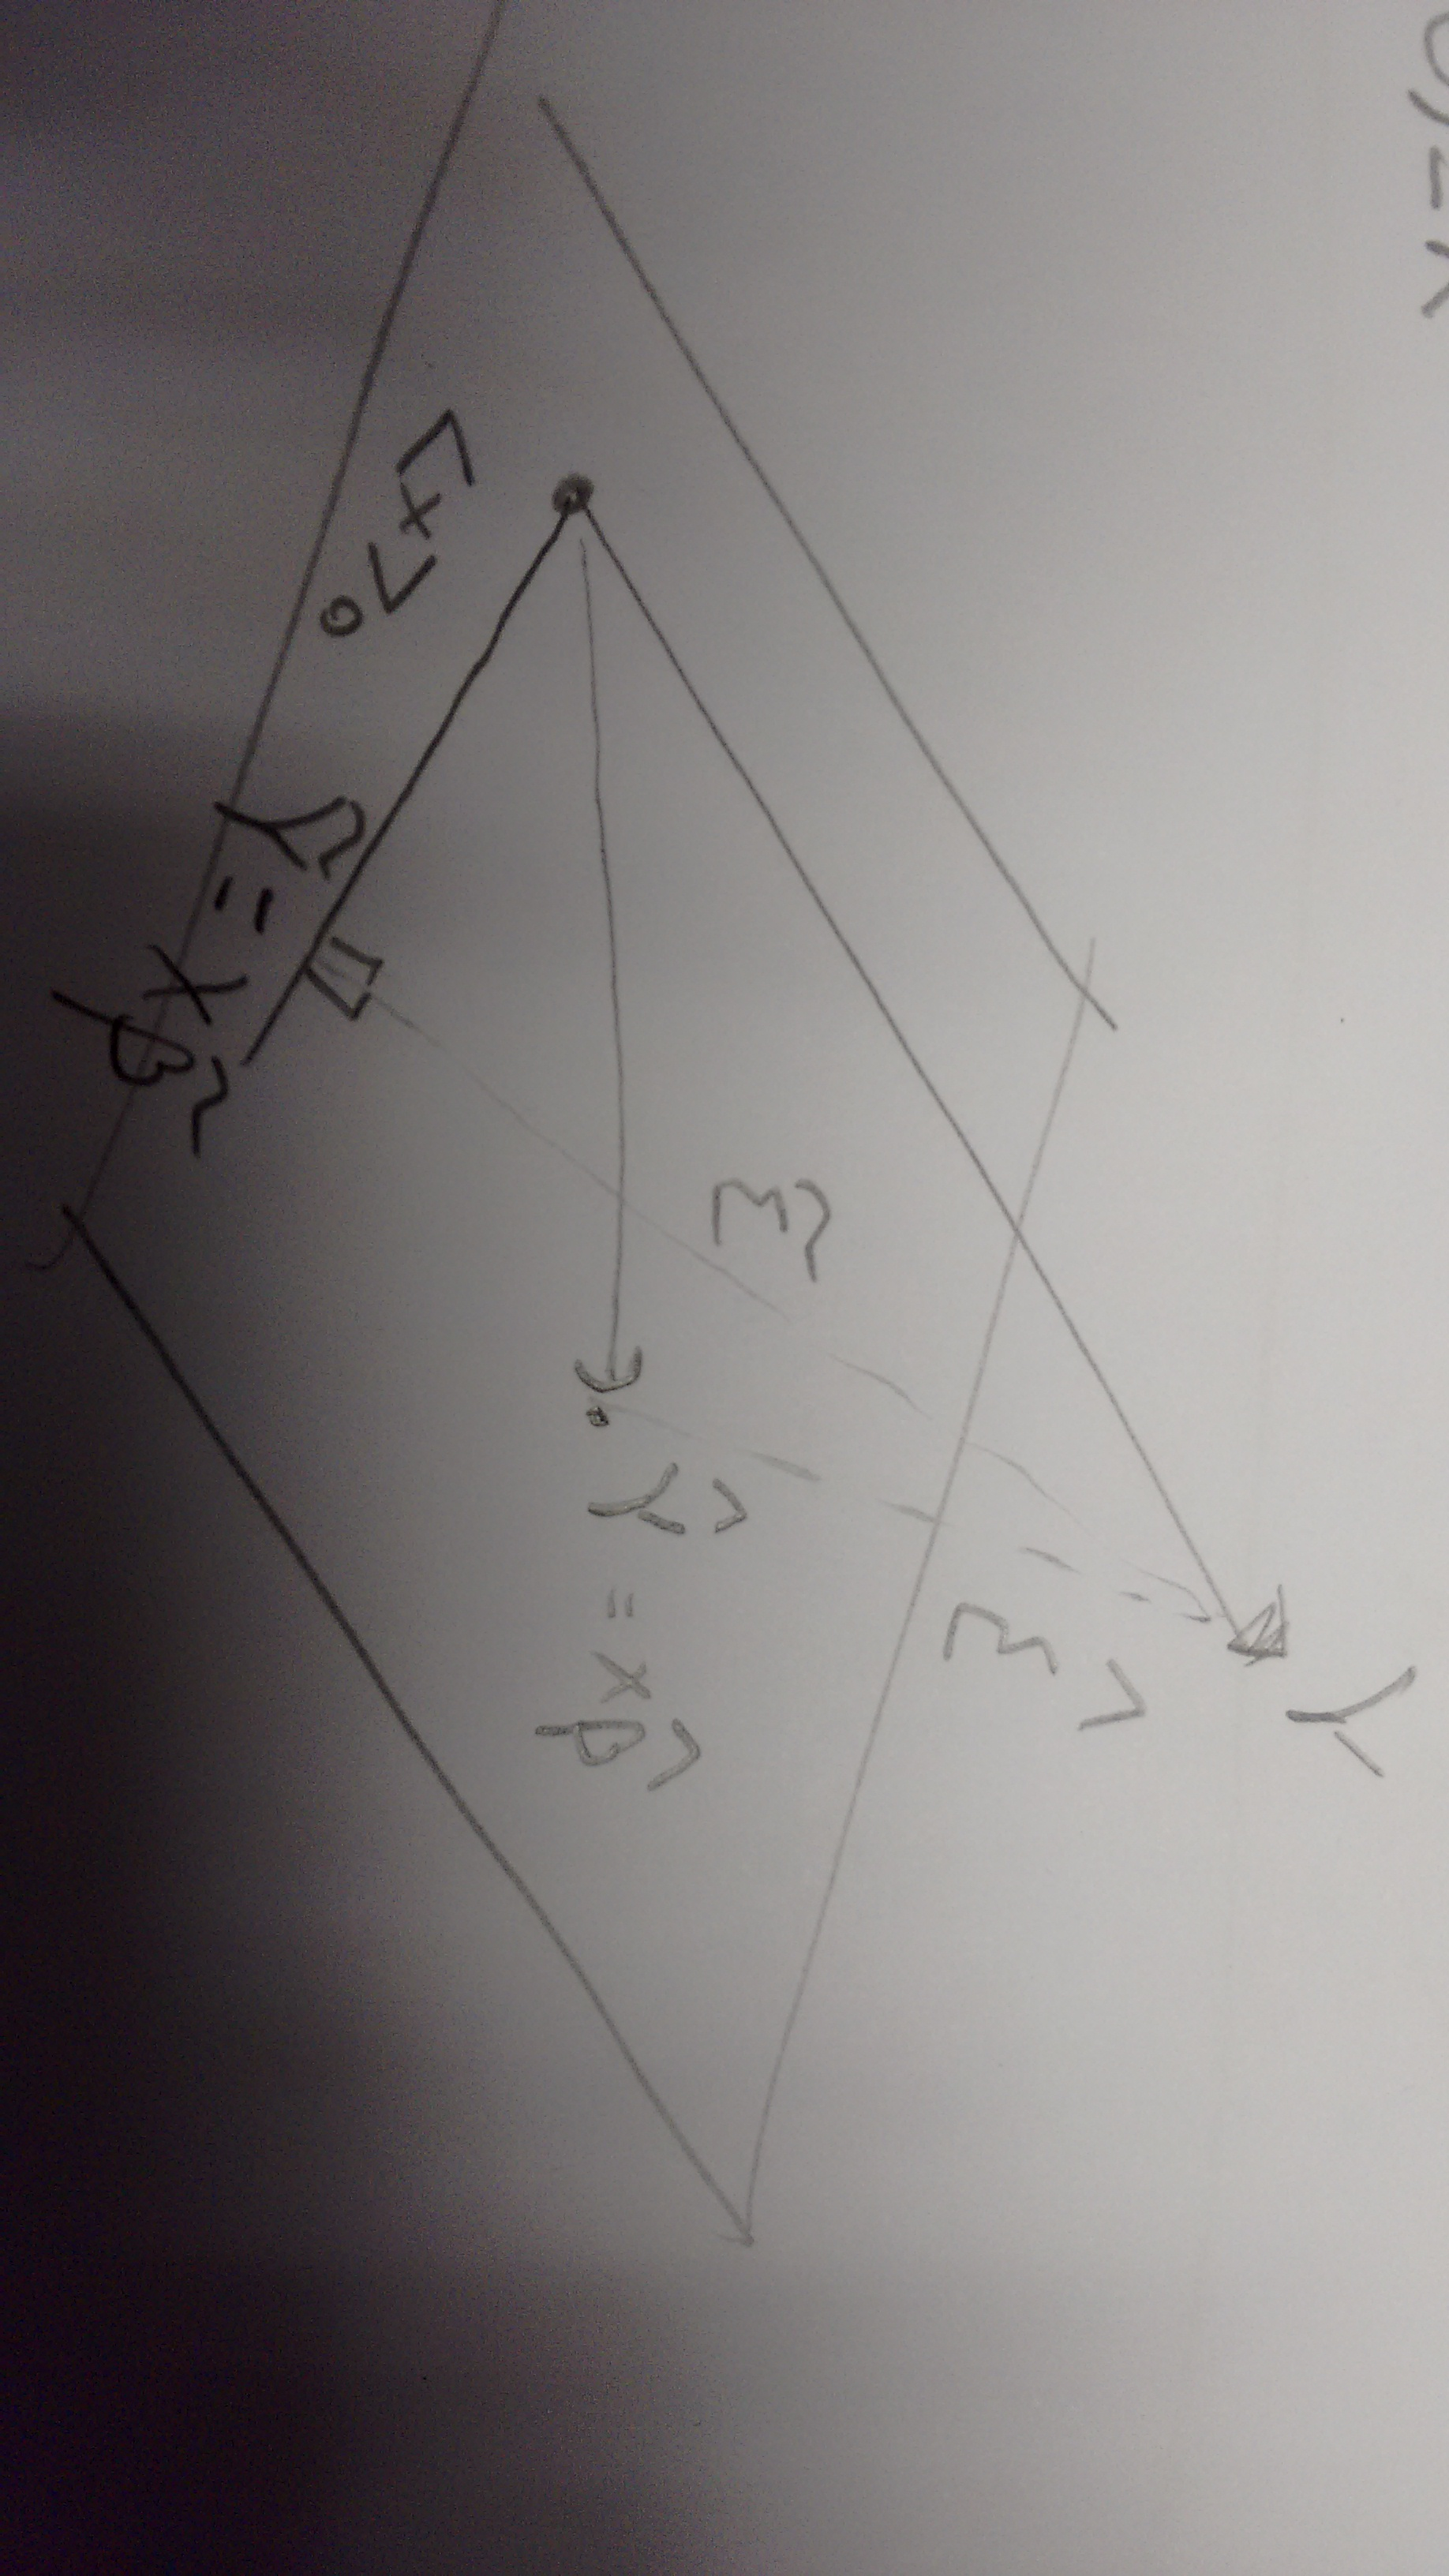
\includegraphics[scale=0.1]{imagenes/ortogonal2.jpg}
\end{center}
\begin{align*}
\hat{\epsilon} = Y - X \hat{\beta}\\
\tilde{\epsilon} = Y - X \tilde{\beta}\\
\hat{\sigma}^2 = \frac{1}{n} ||\hat{\epsilon}||^2\\
\tilde{\sigma}^2 = \frac{1}{n} ||\tilde{\epsilon}||^2\\
\Rightarrow \lambda (y) = \frac{||\tilde{\epsilon}||^2}{||\hat{\epsilon}||^2}
\end{align*}
Cada forma cuadrática en este cuociente es $\chi^2$ pero son dependientes.\\

Vamos a cambiar el cociente usando otras formas cuadráticas de vectores ortogonales y con ello accederemos a una ley sencilla para $\lambda (y)$.\\

Por Pitágoras $||\tilde{\epsilon}||^2 = ||\hat{\epsilon}||^2 + ||\underbrace{\hat{Y}-\tilde{Y}}_{\hat{\epsilon}-\tilde{\epsilon}}||^2$, entonces $\lambda (y) = 1+ \frac{||\hat{\epsilon}-\tilde{\epsilon}||^2}{||\hat{\epsilon}||^2}$\\

Ahora si, las formas cuadráticas $||\tilde{\epsilon}-\hat{\epsilon}||^2$ y $||\hat{\epsilon}||^2$ son variables aleatorias independientes $\chi^2$, con sus grados de libertad.\\

Se puede demostrar que el cociente
\begin{align*}
\frac{||\tilde{\epsilon}-\hat{\epsilon}||^2/(k-p)}{||\hat{\epsilon}||^2/(n-k)}
\end{align*}
tiene ley de Fisher-Snedecor con $(k-q, n-k)$ grados de libertad. Esta ley es conocida y no depende de $\theta = (\beta, \sigma)$. Esto ocurre en el supuesto que $H_{0}\colon H\beta = 0$ sea cierta.

\section{Modelo lineal generalizado}
Pensemos en $Y=X\beta+\epsilon$ con $X$ de rango completo pero $\mathbb{E}(\epsilon\epsilon') \not = \sigma^2I$.\\
En realidad, supongamos que $\mathbb{E}(\epsilon\epsilon') = \sigma^2 \Sigma$, es decir posiblemente con $cov(\epsilon_{i},\epsilon_{j}) \not = 0$.\\

Si estamos en esta situación en el modelo $Y=X\beta + \epsilon$, igual podemos estimar $\beta$ con $\hat{\beta} = (X'X)^{-1}X'Y$. Pero esto no es ``muy buena idea''.\\

Para entender, supongamos que $\Sigma = \begin{bmatrix}
\sigma_{11} 0 \\ 0 \sigma_{22} \\ \ldots \\ 00000000 \sigma_{nn}
\end{bmatrix}$, los errores no son correlacionados pero tienen distintas varianzas.\\

El método clásico dice $\min_{\beta} \sum_{i=1}^{n} \frac{(Y_{i}-\sum_{j=1}^k \beta_{ij} x_{ij})^2}{\sigma_{ii}}$. Sería preferible ponderar por los $\sigma_{ii}^{-1}$\\
%% Suponga que la varianza es cero entonces algo con esto
El problema más grave es que el teorema de Gauss-Markov no se cumple $\mathbb{E}(\epsilon\epsilon') = \sigma^2I$, lo que se hace es transformar el modelo linealmente. Sea $A$ una matriz apropiada y multipliquemos el modelo por A, es decir de $Y=X\beta+\epsilon$ pasamos a $AY = AX\beta + A\epsilon = Z = U\beta + \delta$.\\

Veamos el vector de errores $\delta$:
\begin{align*}
\mathbb{E}(\delta) = \mathbb{E}(A\epsilon) = A\mathbb{E}(\epsilon) = 0\\
\mathbb{V}(\delta) = \mathbb{V}(A\epsilon) = A\mathbb{V}(\epsilon)A' = A\Sigma A'
\end{align*}
Existe $A$ tal que $A\Sigma A' = I$? Esta matriz existe y podemos entenderla como la raíz de $\Sigma$.\\

Usando $A$ con esta propiedad resulta que el modelo $Z=U\beta + \delta$ satisface las hipótesis de Gauss-Markov y podemos calcular
\begin{align*}
\hat{\beta}_{G} = (\underbrace{U'U}_{X'A'AX})^{-1}\underbrace{U'Z}_{X'A'AY = X'\Sigma Y}\\
\Rightarrow \hat{\beta}_{G} = (X'\Sigma^{-1}X)^{-1}X'\Sigma^{1}Y
\end{align*}
y tenemos también $\hat{\beta} = (X'X)^{-1}XY$
\end{document}
